% 若编译失败,且生成 .synctex(busy) 辅助文件,可能有两个原因:
% 1. 需要插入的图片不存在:Ctrl + F 搜索 'figure' 将这些代码注释/删除掉即可
% 2. 路径/文件名含中文或空格:更改路径/文件名即可

% --------------------- 文章宏包及相关设置 --------------------- %
% >> ------------------ 文章宏包及相关设置 ------------------ << %
% 设定文章类型与编码格式
\documentclass[zihao=-4, UTF8]{article}		% 设置全文字号大小, -4 为小四, 5 为五号

% 本文特殊宏包

% 自定义宏定义
    \def\N{\mathbb{N}}
    \def\F{\mathbb{F}}
    \def\Z{\mathbb{Z}}
    \def\Q{\mathbb{Q}}
    \def\R{\mathbb{R}}
    \def\C{\mathbb{C}}
    \def\T{\mathbb{T}}
    \def\S{\mathbb{S}}
    \def\A{\mathbb{A}}
    \def\I{\mathscr{I}}
    \def\d{\mathrm{d}}
    \def\p{\partial}


% 导入基本宏包
    \usepackage[UTF8]{ctex}     % 设置文档为中文语言
        \usepackage{hyperref}  % 宏包:自动生成超链接 (此宏包与标题中的数学环境冲突)
    \hypersetup{
        colorlinks=true,    % false:边框链接 ; true:彩色链接
        citecolor={blue},    % 文献引用颜色
        linkcolor={blue},   % 目录 (我们在目录处单独设置),公式,图表,脚注等内部链接颜色
        urlcolor={magenta},    % 网页 URL 链接颜色,包括 \href 中的 text
        % cyan 浅蓝色 
        % magenta 洋红色
        % yellow 黄色
        % black 黑色
        % white 白色
        % red 红色
        % green 绿色
        % blue 蓝色
        % gray 灰色
        % darkgray 深灰色
        % lightgray 浅灰色
        % brown 棕色
        % lime 石灰色
        % olive 橄榄色
        % orange 橙色
        % pink 粉红色
        % purple 紫色
        % teal 蓝绿色
        % violet 紫罗兰色
    }
    % \usepackage{docmute}    % 宏包:子文件导入时自动去除导言区,用于主/子文件的写作方式,\include{./51单片机笔记}即可。注:启用此宏包会导致.tex文件capacity受限。
    \usepackage{amsmath}    % 宏包:数学公式
    \usepackage{mathrsfs}   % 宏包:提供更多数学符号
    \usepackage{amssymb}    % 宏包:提供更多数学符号
    \usepackage{pifont}     % 宏包:提供了特殊符号和字体
    \usepackage{extarrows}  % 宏包:更多箭头符号
    \usepackage{multicol}   % 宏包:支持多栏 


% 文章页面margin设置
    \usepackage[a4paper]{geometry}
        \geometry{top=2.6cm}  % 1 inch= 2.46 cm, 0.75 inch = 1.85 cm
        \geometry{bottom=2.6cm}
        \geometry{left=2.55cm}
        \geometry{right=2.55cm}   % 设置上下左右页边距
        \geometry{marginparwidth=1.75cm}    % 设置边注距离(注释、标记等)

% 配置数学环境
    \usepackage{amsthm} % 宏包:数学环境配置
    % theorem-line 环境自定义
        \newtheoremstyle{MyLineTheoremStyle}% <name>
            {11pt}% <space above>
            {11pt}% <space below>
            {\kaishu}% <body font> 使用默认正文字体
            {}% <indent amount>
            {\bfseries}% <theorem head font> 设置标题项为加粗
            {:}% <punctuation after theorem head>
            {.5em}% <space after theorem head>
            {\textbf{#1}\thmnumber{#2}\ \ (\,\textbf{#3}\,)}% 设置标题内容顺序
        \theoremstyle{MyLineTheoremStyle} % 应用自定义的定理样式
        \newtheorem{LineTheorem}{Theorem.\,}
    % theorem-block 环境自定义
        \newtheoremstyle{MyBlockTheoremStyle}% <name>
            {11pt}% <space above>
            {11pt}% <space below>
            {\kaishu}% <body font> 使用默认正文字体
            {}% <indent amount>
            {\bfseries}% <theorem head font> 设置标题项为加粗
            {:\\ \indent}% <punctuation after theorem head>
            {.5em}% <space after theorem head>
            {\textbf{#1}\thmnumber{#2}\ \ (\,\textbf{#3}\,)}% 设置标题内容顺序
        \theoremstyle{MyBlockTheoremStyle} % 应用自定义的定理样式
        \newtheorem{BlockTheorem}[LineTheorem]{Theorem.\,} % 使用 LineTheorem 的计数器
    % definition 环境自定义
        \newtheoremstyle{MySubsubsectionStyle}% <name>
            {11pt}% <space above>
            {11pt}% <space below>
            {}% <body font> 使用默认正文字体
            {}% <indent amount>
            {\bfseries}% <theorem head font> 设置标题项为加粗
            {:\\ \indent}% <punctuation after theorem head>
            {0pt}% <space after theorem head>
            {\textbf{#3}}% 设置标题内容顺序
        \theoremstyle{MySubsubsectionStyle} % 应用自定义的定理样式
        \newtheorem{definition}{}

%宏包:有色文本框(proof环境)及其设置
    \usepackage[dvipsnames,svgnames]{xcolor}    %设置插入的文本框颜色
    \usepackage[strict]{changepage}     % 提供一个 adjustwidth 环境
    \usepackage{framed}     % 实现方框效果
        \definecolor{graybox_color}{rgb}{0.95,0.95,0.96} % 文本框颜色。修改此行中的 rgb 数值即可改变方框纹颜色,具体颜色的rgb数值可以在网站https://colordrop.io/ 中获得。(截止目前的尝试还没有成功过,感觉单位不一样)(找到喜欢的颜色,点击下方的小眼睛,找到rgb值,复制修改即可)
        \newenvironment{graybox}{%
        \def\FrameCommand{%
        \hspace{1pt}%
        {\color{gray}\small \vrule width 2pt}%
        {\color{graybox_color}\vrule width 4pt}%
        \colorbox{graybox_color}%
        }%
        \MakeFramed{\advance\hsize-\width\FrameRestore}%
        \noindent\hspace{-4.55pt}% disable indenting first paragraph
        \begin{adjustwidth}{}{7pt}%
        \vspace{2pt}\vspace{2pt}%
        }
        {%
        \vspace{2pt}\end{adjustwidth}\endMakeFramed%
        }

% 外源代码插入设置
    % matlab 代码插入设置
    \usepackage{matlab-prettifier}
        \lstset{style=Matlab-editor}    % 继承 matlab 代码高亮 , 此行不能删去
    \usepackage[most]{tcolorbox} % 引入tcolorbox包 
    \usepackage{listings} % 引入listings包
        \tcbuselibrary{listings, skins, breakable}
        \newfontfamily\codefont{Consolas} % 定义需要的 codefont 字体
        \lstdefinestyle{MatlabStyle_inc}{   % 插入代码的样式
            language=Matlab,
            basicstyle=\small\ttfamily\codefont,    % ttfamily 确保等宽 
            breakatwhitespace=false,
            breaklines=true,
            captionpos=b,
            keepspaces=true,
            numbers=left,
            numbersep=15pt,
            showspaces=false,
            showstringspaces=false,
            showtabs=false,
            tabsize=2,
            xleftmargin=15pt,   % 左边距
            %frame=single, % single 为包围式单线框
            frame=shadowbox,    % shadowbox 为带阴影包围式单线框效果
            %escapeinside=``,   % 允许在代码块中使用 LaTeX 命令 (此行无用)
            %frameround=tttt,    % tttt 表示四个角都是圆角
            framextopmargin=0pt,    % 边框上边距
            framexbottommargin=0pt, % 边框下边距
            framexleftmargin=5pt,   % 边框左边距
            framexrightmargin=5pt,  % 边框右边距
            rulesepcolor=\color{red!20!green!20!blue!20}, % 阴影框颜色设置
            %backgroundcolor=\color{blue!10}, % 背景颜色
        }
        \lstdefinestyle{MatlabStyle_src}{   % 插入代码的样式
            language=Matlab,
            basicstyle=\small\ttfamily\codefont,    % ttfamily 确保等宽 
            breakatwhitespace=false,
            breaklines=true,
            captionpos=b,
            keepspaces=true,
            numbers=left,
            numbersep=15pt,
            showspaces=false,
            showstringspaces=false,
            showtabs=false,
            tabsize=2,
        }
        \newtcblisting{matlablisting}{
            %arc=2pt,        % 圆角半径
            % 调整代码在 listing 中的位置以和引入文件时的格式相同
            top=0pt,
            bottom=0pt,
            left=-5pt,
            right=-5pt,
            listing only,   % 此句不能删去
            listing style=MatlabStyle_src,
            breakable,
            colback=white,   % 选一个合适的颜色
            colframe=black!0,   % 感叹号后跟不透明度 (为 0 时完全透明)
        }
        \lstset{
            style=MatlabStyle_inc,
        }

% table 支持
    \usepackage{booktabs}   % 宏包:三线表
    \usepackage{tabularray} % 宏包:表格排版
    \usepackage{longtable}  % 宏包:长表格

% figure 设置
    \usepackage{graphicx}  % 支持 jpg, png, eps, pdf 图片 
    \usepackage{svg}       % 支持 svg 图片
        \svgsetup{
            % 指向 inkscape.exe 的路径
            inkscapeexe = C:/aa_MySame/inkscape/bin/inkscape.exe, 
            % 一定程度上修复导入后图片文字溢出几何图形的问题
            inkscapelatex = false                 
        }

% 图表进阶设置
    \usepackage{caption}    % 图注、表注
        \captionsetup[figure]{name=图}  
        \captionsetup[table]{name=表}
        \captionsetup{
            labelfont=bf, % 设置标签为粗体
            textfont=bf,  % 设置文本为粗体
            font=small  
        }
    \usepackage{float}     % 图表位置浮动设置 

% 圆圈序号自定义
    \newcommand*\circled[1]{\tikz[baseline=(char.base)]{\node[shape=circle,draw,inner sep=0.8pt, line width = 0.03em] (char) {\small \bfseries #1};}}   % TikZ solution

% 列表设置
    \usepackage{enumitem}   % 宏包:列表环境设置
        \setlist[enumerate]{itemsep=0pt, parsep=0pt, topsep=0pt, partopsep=0pt, leftmargin=3.5em} 
        \setlist[itemize]{itemsep=0pt, parsep=0pt, topsep=0pt, partopsep=0pt, leftmargin=3.5em}
        \newlist{circledenum}{enumerate}{1} % 创建一个新的枚举环境  
        \setlist[circledenum,1]{  
            label=\protect\circled{\arabic*}, % 使用 \arabic* 来获取当前枚举计数器的值,并用 \circled 包装它  
            ref=\arabic*, % 如果需要引用列表项,这将决定引用格式(这里仍然使用数字)
            itemsep=0pt, parsep=0pt, topsep=0pt, partopsep=0pt, leftmargin=3.5em
        }  

% 其它设置
    % 脚注设置
        \renewcommand\thefootnote{\ding{\numexpr171+\value{footnote}}}
    % 参考文献引用设置
        \bibliographystyle{unsrt}   % 设置参考文献引用格式为unsrt
        \newcommand{\upcite}[1]{\textsuperscript{\cite{#1}}}     % 自定义上角标式引用
    % 文档摘要设置
        \newcommand{\cnabstractname}{\large 摘要}
        \newenvironment{cnabstract}{%
        \par
        \noindent\mbox{}\hfill{\bfseries \cnabstractname}\hfill\mbox{}\par
        }{\par}

% 文章默认字体设置
\usepackage{fontspec}   % 宏包:字体设置
    \setmainfont{SimSun}    % 设置中文字体为宋体字体
    \setCJKmainfont[AutoFakeBold=3]{SimSun} % 设置加粗字体为 SimSun 族,AutoFakeBold 可以调整字体粗细
    \setmainfont{Times New Roman} % 设置英文字体为Times New Roman

% 各级标题自定义设置
\usepackage{titlesec} % 宏包:各级标题设置
\usepackage{titling}  % 宏包:标题设置
\setlength{\droptitle}{-2.6cm}  % 调整标题位置
\pretitle{\begin{center}\LARGE}
\posttitle{\end{center}}
% section标题自定义设置 
\titleformat{\section}{\Large\centering\bfseries}{\thesection.}{1em}{}
\titleformat{\subsection}{\normalsize\large\bfseries}{\thesubsection}{1em}{}
\titleformat{\subsubsection}{\normalsize\bfseries}{\thesubsubsection}{1em}{}
% subsubsection标题自定义设置
%\titleformat{\subsubsection}[hang]{\normalfont\bfseries}{}{8pt}{}

% --------------------- 文章宏包及相关设置 --------------------- %
% >> ------------------ 文章宏包及相关设置 ------------------ << %

% ------------------------ 文章信息区 ------------------------ %
% ------------------------ 文章信息区 ------------------------ %
% 页眉页脚设置
    %\usepackage{fancyhdr}   %宏包:页眉页脚设置
    %    \pagestyle{fancy}
    %    \fancyhf{}
    %    \cfoot{\thepage}
    %    \renewcommand\headrulewidth{1pt}
    %    \renewcommand\footrulewidth{0pt}
    %    \usepackage{fontawesome}    % 宏包:更多符号与图标 (用于插入 GitHub 图标等)
        \lhead{\small
        \href{https://github.com/YiDingg/LatexNotes}{\color{black}\faGithub\ https://github.com/YiDingg/LatexNotes}
        } 
    %    \chead{here is the header,这里是页眉}    
    %    \rhead{\small dingyi233@mails.ucas.ac.cn}
%文档信息设置
    \title{\textbf{这里是标题}}
    \author{ }  % 必须为空
    \date{ }  % 必须为空
% ------------------------ 文章信息区 ------------------------ %
% ------------------------ 文章信息区 ------------------------ %

% 开始编辑文章

\begin{document} 

\maketitle
%\thispagestyle{fancy}
\vspace{-80pt}

\begin{cnabstract}{\normalsize 

定日镜场能将太阳光反射汇聚到安装在镜场中的吸收塔集热器上,实现能量转换,
不同的定日镜场参数会影响定日镜场的效率。本文通过光线反射、入射等模型,计算
给定参数下的定日镜场效率,并建立定日镜场的效率优化模型,研究定日镜场参数变
化对单位镜面面积平均输出热功率的影响。 

\textbf{针对问题一},本文建立了\textbf{定日镜场的效率计算模型}。首先,建立镜场大地坐标系、
镜面坐标系和光锥束坐标系,描述定日镜场的参数。太阳光束的入射光线和反射光线
考虑为光锥束,计算太阳光的入射和反射,考虑阴影遮挡损失、余弦损失、集热器截
断效率等因素。通过\textbf{坐标变换和方程联立},判断某入射光线及对应的反射光线是否造
成阴影遮挡损失所涉及的各种损失,再
判断成功反射出的光线是否被集热器接收。最后得到光学效率和输出热功率的表达式,
进一步计算各个效率和功率等。在
某个定日镜上取点步长τ 为 1m,在光锥束上取 1 θ = 0.002rad , 2 θ = 0,π / 2,π ,3π / 2,进行网格化构建入射光线束和反射光线束,计算得到表 1 和表 2。该定日镜场的\textbf{年平均输出光学效率 $0.536230167$}、\textbf{年平均输出热功率 32.76117051 $\mathbf{MW}$}、\textbf{单位镜面面积年平均输出热功率 0.521508604 $\mathbf{KW\cdot m^{-2}}$},最后,进行敏感性分析,分析步长 $\tau$ 对结果的影响。 

\textbf{针对问题二},本文提出了\textbf{单位镜面面积年平均输出热功率的优化模型}。问题二是
在定日镜场的额定年平均输出热功率为 60MW 的条件下,设计定日镜场的参数,使得
单位镜面面积年平均输出热功率尽量大。\textbf{决策变量}包括吸收塔的位置坐标、定日镜的
尺寸(相同)、安装高度、数量和位置。\textbf{目标函数}是单位镜面面积年平均输出热功率的
最大值,\textbf{约束条件}包括镜面边长在 2m 至 8m 之间、安装高度在 2m 至 6m 之间、相邻
定日镜底座中心距离比镜面宽度多 5m 等。先取 w,v 相等,用\textbf{蜂窝排列法}确定圆环内能
排列的定日镜数目和位置。然后将蜂窝进行绕原点旋转 µ ,用蒙特卡洛模拟法对部分
定日镜进行随机抽样,得到粗决策变量,从而进一步计算光学效率和单位面积输出热
功率等。最后遍历 $\mu, w = \nu, \tilde{h}, X_0, Y_0 $ 寻找决策变量的最优解。得到该定日镜场的\textbf{年平均输出光学效率 0.591643667}、\textbf{年平均输出热功率68.24427914 $\  \mathbf{MW}$}、\textbf{单位镜面面积年平均输出热功率  0.572538333 $  \mathbf{KW\cdot m^{-2}}$ }

\textbf{针对问题三},本文提出了\textbf{单位镜面面积年平均输出热功率的优化模型}。问题三是
在\textbf{定日镜尺寸和安装高度可以不同}的情况下,设计定日镜场的参数,使得单位镜面面
积年平均输出热功率尽量大。以\textbf{单位镜面面积年平均输出热功率}为目标函数,以吸收
塔位置坐标、定日镜尺寸、安装高度、定日镜数目、定日镜位置为决策变量,以额定
功率、相邻定日镜距离、圆形区域半径等为约束条件,建立优化模型。考虑通过第二
问求得结果进一步优化,将最外围的定日镜安装高度升高为 6m,其他不变,得到该定
日镜场的\textbf{年平均输出光学效率 0.496428083}、\textbf{年平均输出热功率 60.336111} $\mathbf{MW}$、\textbf{单位
镜面面积年平均输出热功率 0.506192417} $\mathbf{KW \cdot m^{-2}}$  
}\par
\vspace{12pt}
{\normalsize \textbf{关键词:坐标旋转,光学效率,输出热功率,锥形光束,蜂窝排列法}}
\end{cnabstract}



\setlength{\parindent}{2em}

\newpage
\section{问题重述}
\subsection{问题背景:}
我查查查资料,然后说哇这个问题背景多好,多有研究意义,简直太棒了太棒了太棒了太棒了太棒了太棒了太棒了太棒了太棒了太棒了太棒了太棒了太棒了太棒了太棒了太棒了太棒了太棒了太棒了太棒了太棒了太棒了太棒了太棒了太棒了太棒了太棒了太棒了太棒了太棒了
\subsection{问题提出(题目重述):}
我重述重述再重述我重述重述再重述我重述重述再重述我重述重述再重述\par
根据上面的信息,我们提出以下几个问题:\par
\textbf{问题一:}这里是问题一\par
\textbf{问题二:}这里是问题二\par
\textbf{问题三:}这里是问题三\par
\textbf{问题四:}这里是问题四\par

\section{问题分析}
\subsection{问题一分析:}
这里我们分析问题一,提出我们将要的模型,给出解决问题的步骤,可以适当增加流程图、有利于问题分析的图像等(物理图解可以用PPT画,也可以用vscode插件draw.io画)。
\subsection{问题二分析:}
这里我们分析问题二,提出我们将要的模型,给出解决问题的步骤
\subsection{问题三分析:}
这里我们分析问题三,提出我们将要的模型,给出解决问题的步骤
\subsection{问题四分析:}
这里我们分析问题四,提出我们将要的模型,给出解决问题的步骤

\section{模型假设}
假设1:巴拉巴拉\par
假设2:巴拉巴拉\par
假设3:巴拉巴拉\par
假设4:芭芭拉巴拉\par
假设5:巴拉巴拉

\section{符号说明}
\begin{table}[ht]
  \centering
  \caption{\textbf{符号含义与约定}}
  \label{tab:waterpump}
  \begin{tabular}{ccccc}
  \toprule
  符号 & 含义& 量纲\\
  \midrule
  符号1& 含义1& 量纲1\\
  符号2& 含义2& 量纲2\\
  符号3& 含义3& 量纲3\\
  符号4& 含义4& 量纲4\\
  \bottomrule
  \end{tabular}
\end{table}

\section{模型建立与求解}

\subsection{问题一:}
\subsubsection{模型建立:}
巴拉巴拉巴拉巴拉巴拉巴拉

\begin{figure}[H]
  \centering
  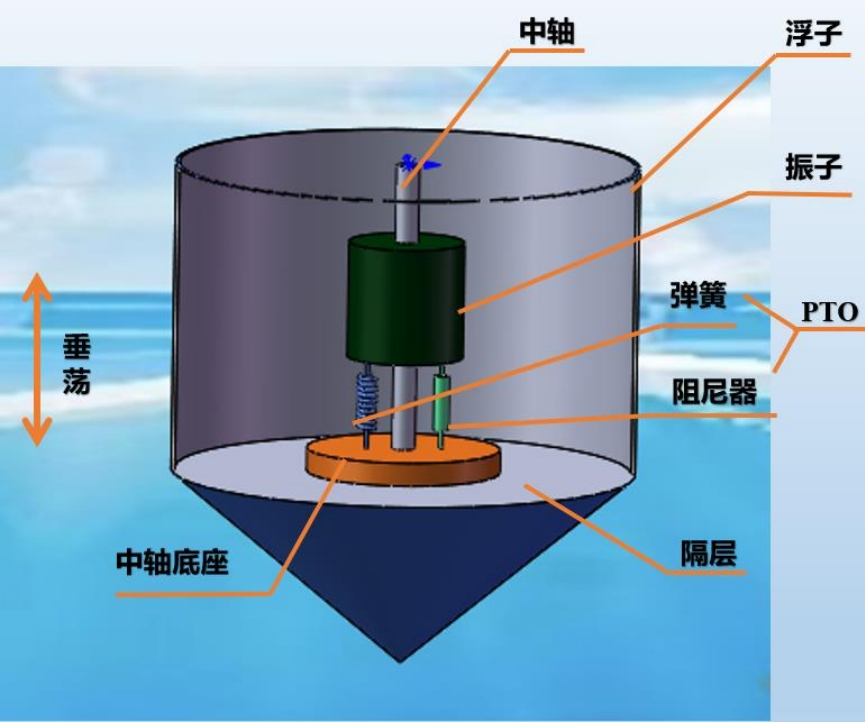
\includegraphics[width=0.6\textwidth]{assets/波浪能装置示意图.jpg}
  \caption{\textbf{插入 jpg}}\label{插入 jpg}
\end{figure}
啊?
\begin{figure}[H]
  \centering
  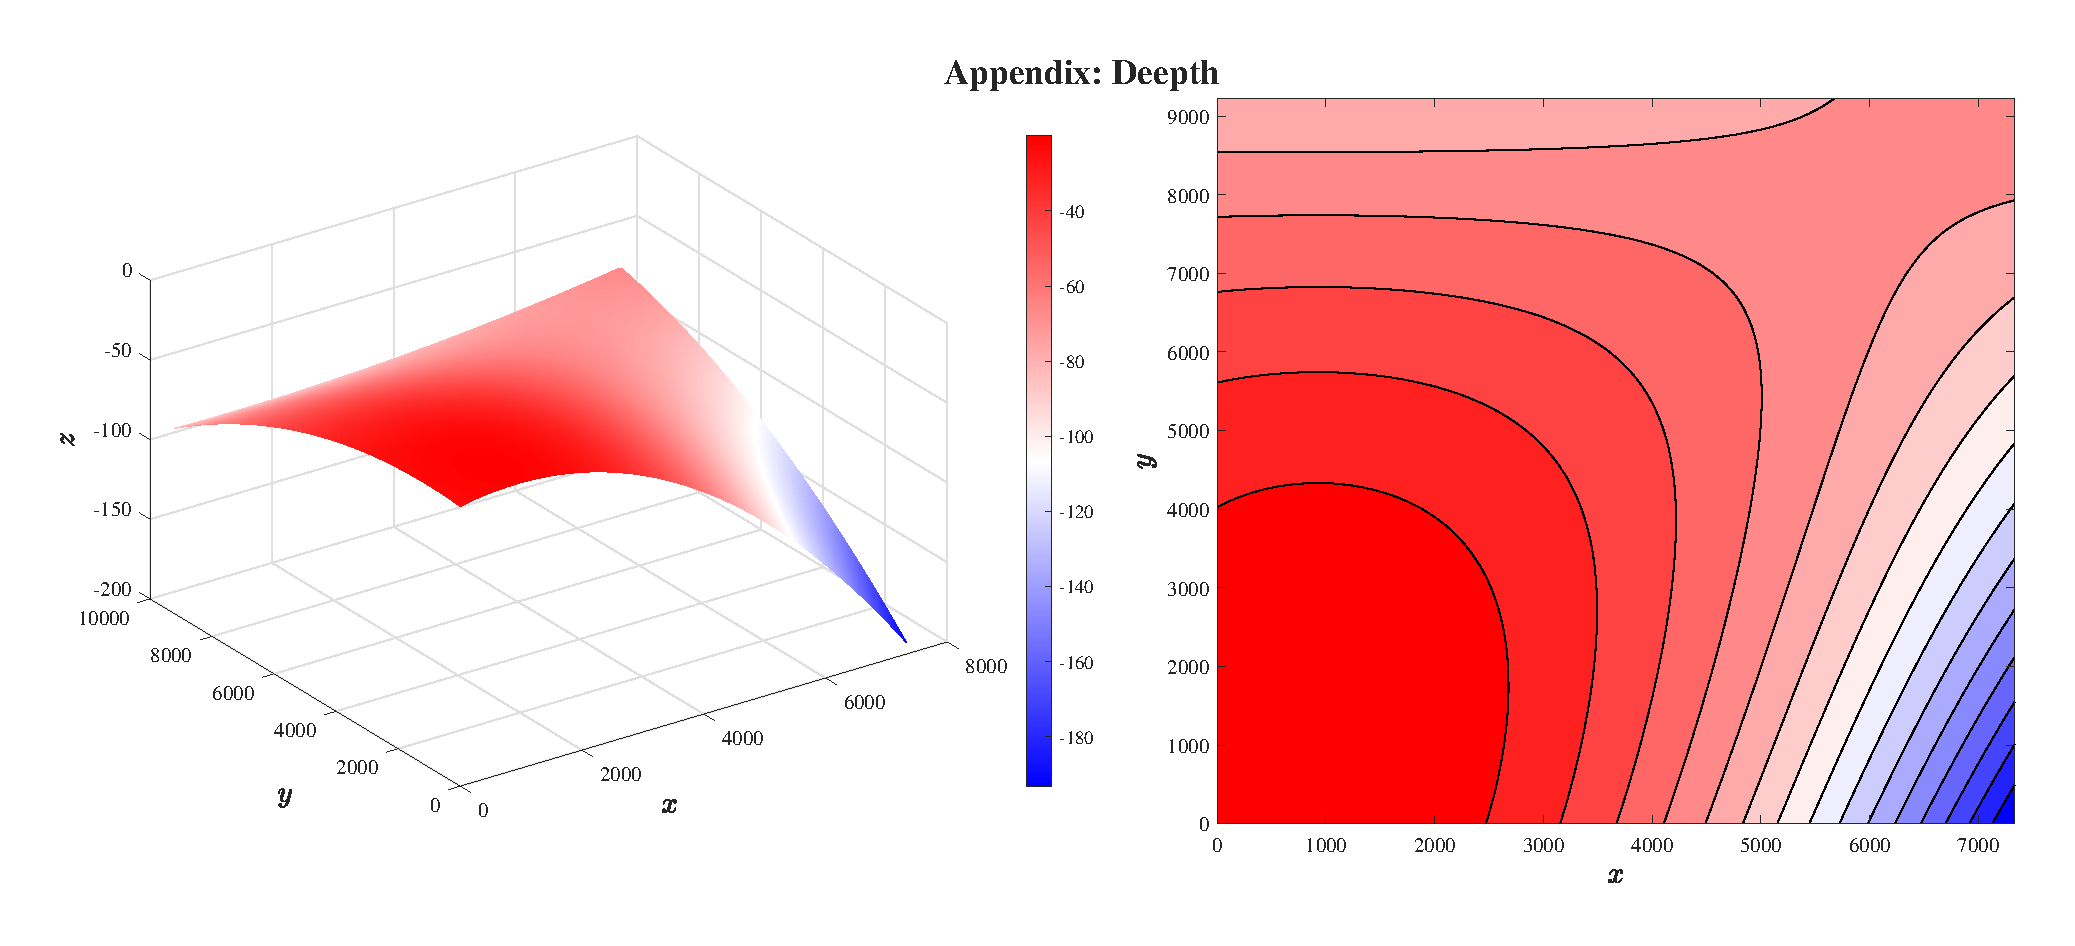
\includegraphics[width=\textwidth]{assets/2024-08-15_02-04-29.pdf}
  \caption{\textbf{插入 pdf}}\label{插入 pdf}
\end{figure}

\subsubsection{模型优化(如果可以优化的话):}
\subsubsection{模型求解:}
\subsubsection{求解结果:}
\subsubsection{可靠性检验:}

\subsection{问题二:}
\subsubsection{模型建立:}
使用巴拉巴拉
\subsubsection{模型求解:}

\begin{figure}[H]
  \centering
  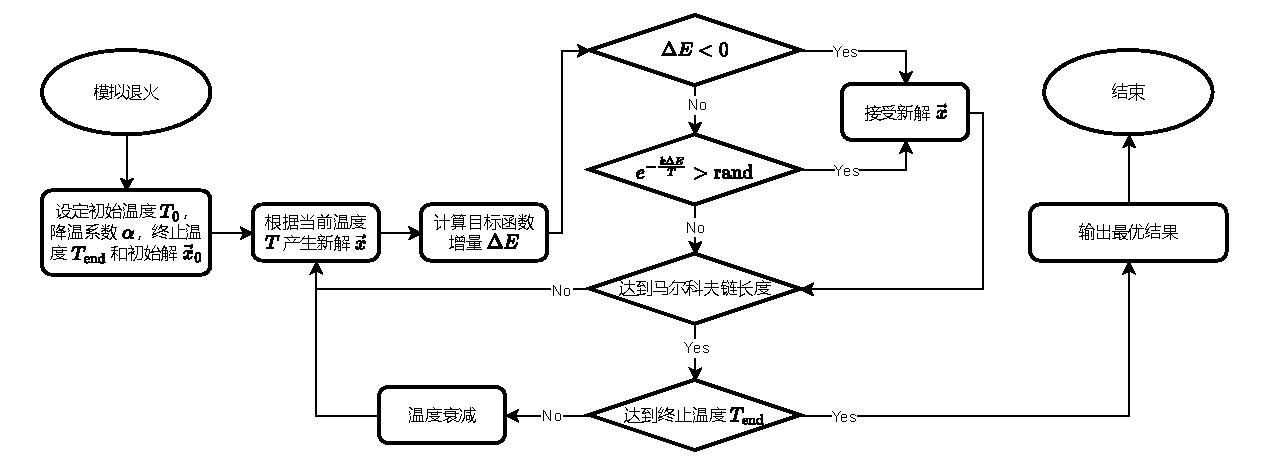
\includegraphics[width=\textwidth]{assets/模拟退火流程图.drawio.pdf}
  \caption{\textbf{模拟退火流程图}}\label{模拟退火流程图}
\end{figure}

\begin{figure}[H]
  \centering
  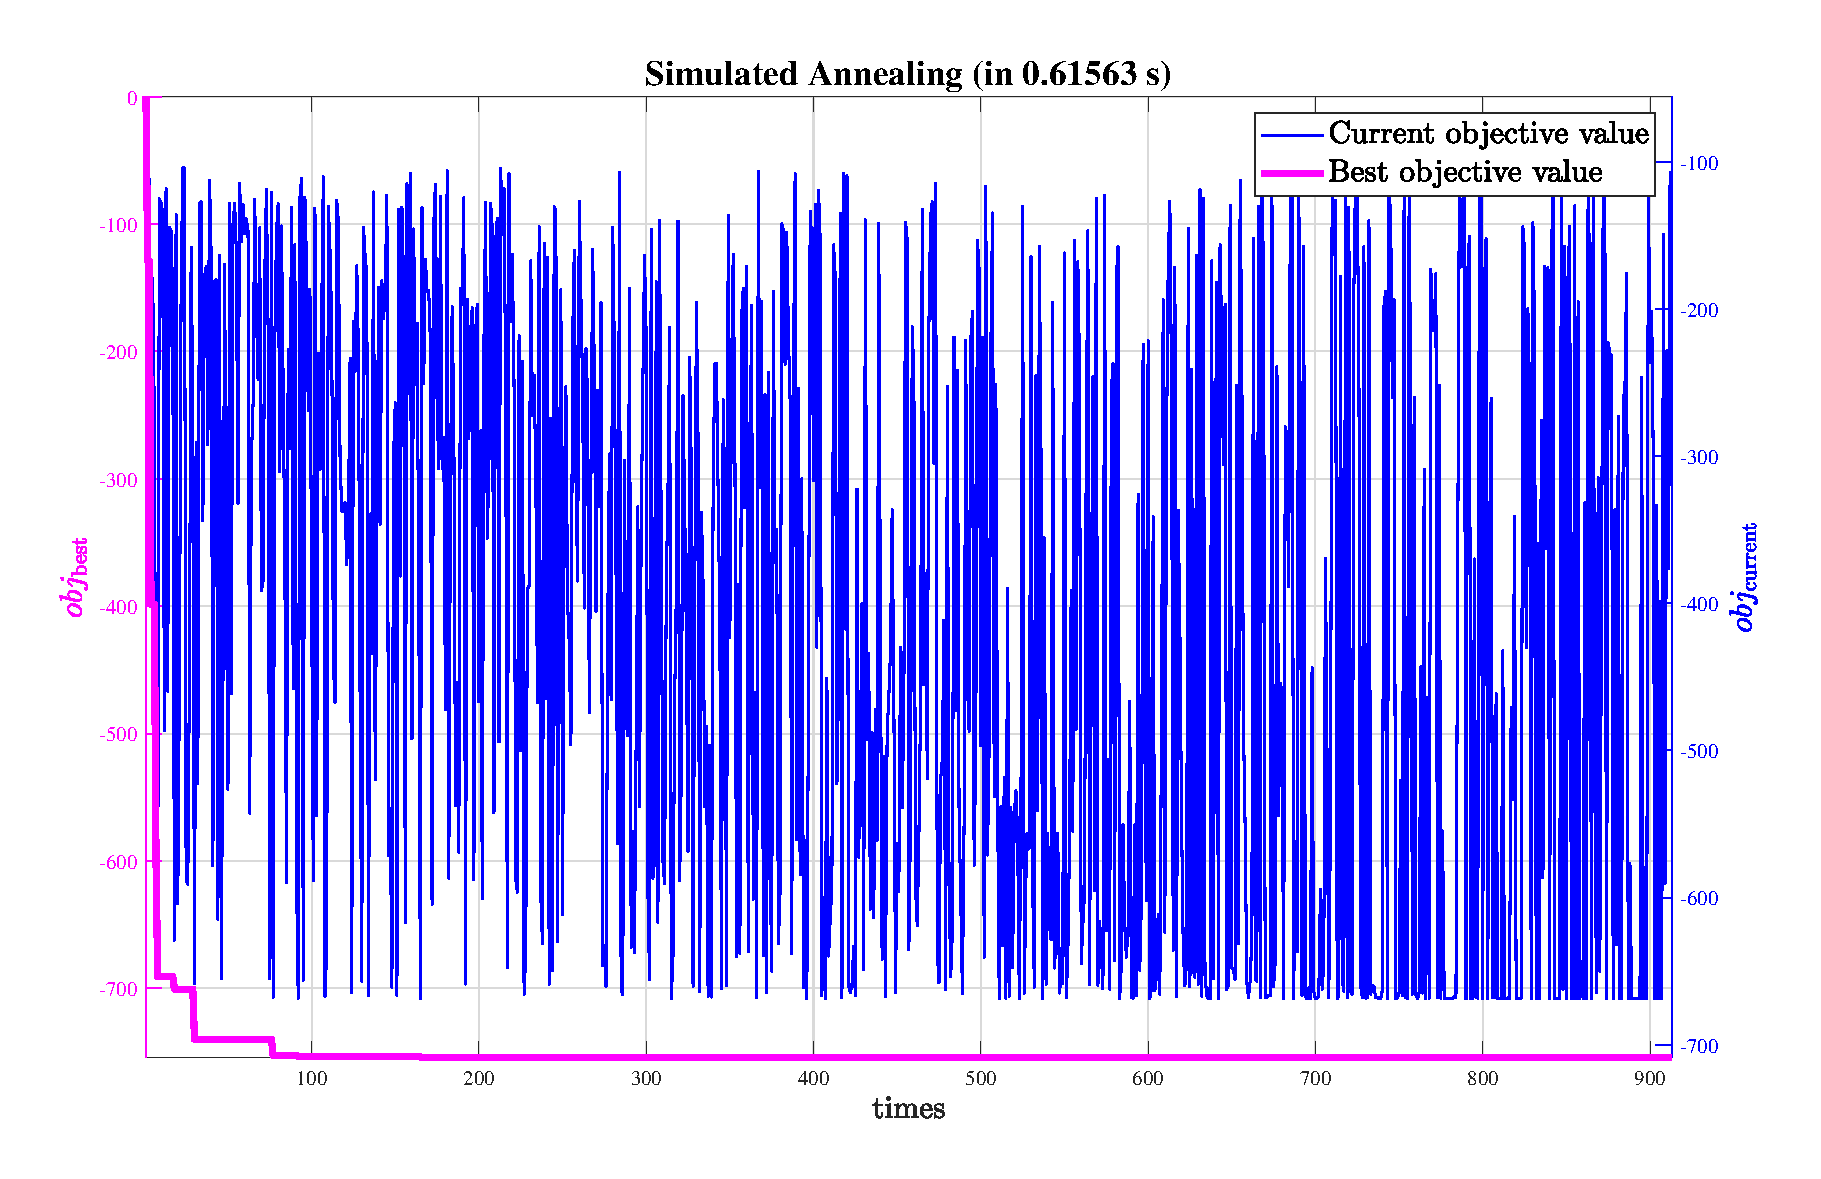
\includegraphics[width=\textwidth]{assets/2024-08-15_13-50-23.pdf}
  \caption{\textbf{模拟退火结果}}\label{模拟退火结果}
\end{figure}

\subsubsection{求解结果:}
\subsubsection{可靠性检验:}

\subsection{问题三:}
\subsubsection{模型建立:}
使用巴拉巴拉
\subsubsection{模型求解:}
\subsubsection{求解结果:}
\subsubsection{可靠性检验:}

\subsection{问题四:}
\subsubsection{模型建立:}
使用巴拉巴拉
\subsubsection{模型求解:}
我解解解解解解解解解解解解解解解解解解解解 \upcite{徐晓平}
\subsubsection{求解结果:}
这里是我们的求解结果 \upcite{张春琳}
\subsubsection{可靠性检验:}

\section{模型评价与推广}
\subsection{模型优点:}
\subsubsection{优点一:}
\subsubsection{优点二:}
\subsection{模型缺点:}
\subsubsection{缺点一:}
\subsubsection{缺点二:}
\subsection{模型推广:}

\nocite{*}
\bibliography{re}
\addcontentsline{toc}{section}{参考文献}


\newpage
\appendix
\titleformat{\section}{\large\centering\bfseries}{附录\thesection.}{1em}{}
\titleformat{\subsection}{\normalsize\bfseries}{\thesubsection}{1em}{}

\section{支撑材料列表}
\begin{center}
  这里插入一张图片(类似思维导图那种)
\end{center}
\section{Matlab 代码}
% 注意:listing环境中手动输入的代码需要顶格写

\begin{matlablisting}
% MATLAB code here
x = 0:0.1:2*pi;
y = sin(x);
plot(x, y);
xlabel('x');
ylabel('sin(x)');
title('Sine Function');
% ... (MATLAB code here,最好是插入文件)
% MATLAB code here
x = 0:0.1:2*pi;
y = sin(x);
plot(x, y);
xlabel('x');
ylabel('sin(x)');
title('Sine Function');
% ... (MATLAB code here,最好是插入文件)
% MATLAB code here
x = 0:0.1:2*pi;
y = sin(x);
plot(x, y);
xlabel('x');
ylabel('sin(x)');
title('Sine Function');
% ... (MATLAB code here,最好是插入文件)
% MATLAB code here
x = 0:0.1:2*pi;
y = sin(x);
plot(x, y);
xlabel('x');
ylabel('sin(x)');
title('Sine Function');
% ... (MATLAB code here,最好是插入文件)
% MATLAB code here
x = 0:0.1:2*pi;
y = sin(x);
plot(x, y);
xlabel('x');
ylabel('sin(x)');
title('Sine Function');
% ... (MATLAB code here,最好是插入文件)
% MATLAB code here
x = 0:0.1:2*pi;
y = sin(x);
plot(x, y);
xlabel('x');
ylabel('sin(x)');
title('Sine Function');
% ... (MATLAB code here,最好是插入文件)% ... (MATLAB code here,最好是插入文件)% ... (MATLAB code here,最好是插入文件)% ... (MATLAB code here,最好是插入文件)% ... (MATLAB code here,最好是插入文件)A
% MATLAB code here
x = 0:0.1:2*pi;
y = sin(x);
plot(x, y);
xlabel('x');
ylabel('sin(x)');
title('Sine Function');
% ... (MATLAB code here,最好是插入文件)
\end{matlablisting}

\section{这里是第三节附录(如果有的话)}

\end{document}

